\section{SOTA of object detection}
\subsection{Introduction to Object Detection}
\href{https://www.mathworks.com/discovery/object-detection.html#:~:text=Object%20detection%20is%20a%20computer,learning%20to%20produce%20meaningful%20results.}{Object detection} is a computer vision technique for locating instances of objects in images or videos. Object detection algorithms typically leverage machine learning or deep learning to produce meaningful results. When humans look at images or videos, we can recognize and locate objects of interest within a matter of moments. The goal of object detection is to replicate this intelligence using a computer. \cite{zhao2019object}, \cite{ansari2020building}
\subsubsection{Why Object Detection}
Object detection is a fundamental task in computer vision that involves identifying and localizing objects within an image or a video. It plays a pivotal role in various real-world applications, contributing to advancements in technology and enhancing our daily lives. The importance of object detection lies in its ability to enable machines to interpret and understand visual information, allowing them to make informed decisions and interact intelligently with the environment.\cite{pathak2018application}, 
\begin{enumerate}
    \item \textbf{Automation and Efficiency:} Object detection is a cornerstone in the development of automated systems, empowering machines to perceive and respond to their surroundings. This is particularly crucial in industries such as manufacturing, where the automation of tasks, such as quality control and inventory management, leads to increased efficiency and reduced operational costs.
    \item \textbf{Enhanced Security and Surveillance:}  In the realm of security and surveillance, object detection is instrumental in identifying potential threats or anomalies. Surveillance cameras equipped with object detection algorithms can automatically detect and alert authorities to suspicious activities, enhancing public safety in crowded spaces, transportation hubs, and critical infrastructure.
    \item \textbf{Autonomous Vehicles:} The advent of autonomous vehicles relies heavily on object detection to interpret the dynamic environment. Cars equipped with object detection systems can identify pedestrians, vehicles, and obstacles, enabling safer navigation and reducing the likelihood of accidents.
    \item \textbf{Medical Imaging and Diagnosis:}  In the field of healthcare, object detection plays a vital role in medical imaging. It aids in the detection and localization of abnormalities in radiological images, facilitating early diagnosis and improving patient outcomes.
    \item \textbf{Retail and Customer Experience:} Object detection is utilized in retail for tasks such as inventory management, shelf monitoring, and cashierless checkout systems. These applications streamline operations and enhance the overall customer experience by reducing waiting times and optimizing stock levels.
\end{enumerate}

\textbf{Real-world Scenarios:}\\
\begin{enumerate}
    \item \textbf{Smart Cities:} object detection is integral to the development of smart cities. In urban environments, it can be used for traffic management, waste management, and monitoring public spaces, contributing to more efficient and sustainable urban living.
    \item \textbf{Search and Rescue Operations:} In disaster-stricken areas, object detection aids in search and rescue operations by identifying and locating individuals in need of assistance. Drones equipped with object detection capabilities can cover large areas quickly, improving the efficiency of rescue efforts.
    \item \textbf{Environmental Monitoring: } Object detection is applied in environmental science for monitoring wildlife, tracking deforestation, and studying biodiversity. It enables researchers to gather crucial data for conservation and ecological studies.
    \item \textbf{Augmented Reality:} Object detection is a key component in augmented reality applications, where virtual elements are seamlessly integrated with the real world. This technology enhances user experiences in gaming, education, and various interactive scenarios.
\end{enumerate} \cite{ansari2020building}, \cite{pathak2018application}

\subsection{Object detection stage}
Object detection can be classified into two stages according to the detection process steps:
\href{https://www.ijert.org/object-detection-using-yolo-and-mobilenet-ssd-a-comparative-study}{\textcolor{blue}{Source}}
\begin{itemize}
    \item \textbf{One-stage detector}  is a simple regression problem that takes input and learns probability classes and bounding box coordinates. YOLO, YOLO v2, SSD, RetinaNet, etc. fall under one-phase detectors. Object detection is an advanced form of imaging classification where a neural network predicts objects in an image and draws attention to them in the form of bounding boxes. \cite{oneStage}
    \item \textbf{Two-stage detector} Where detection is completed in two steps, the first step uses regional design networks to create areas of interest with a high probability of being objects. The second step is object detection, which performs the final classification and regression of the bounding box of the objects. RCNN, Fast RCNN, SPPNET, Faster RCNN, etc., are some of the two-stage detectors. \cite{du2020overview}
\end{itemize}

\begin{figure}[H]
    \centering
    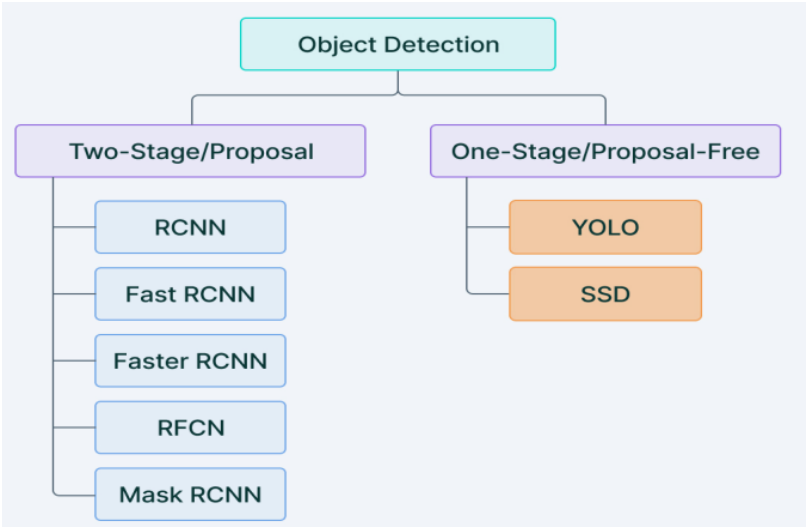
\includegraphics[width=0.7\textwidth]{ObjectDetection_Stage.PNG}
    \caption{Stage  or classification of Object Detection}
    \label{fig:Stage of Object Detection}
\end{figure}

\subsection{Two-Stage/Proposal: }
  Two-stage object detection algorithms typically follow a two-step process: region proposal and object classification or refinement. One of the most popular two-stage object detection frameworks is the region-based Convolutional Neural Network (R-CNN) and its variants. \cite{du2020overview}, \cite{ansari2020building}
\subsubsection{Region-Based Convolutional Neural Network: } \underline{\textcolor{blue}{\href{https://arxiv.org/pdf/1311.2524.pdf}{R-CNN}}}
 A Region-Based Convolutional Neural Network (R-CNN) is a type of convolutional neural network designed for object detection in images.R-CNN predominantly uses region proposals using a selective search (SS) approach to pre-compute the priors. The features between these regions are not shared, so we have to extract features individually for each region-of-interest (RoI) generated using an SS approach. In contrast, R-CNNs are designed to not only classify objects but also to locate and delineate their boundaries within the image.
The R-CNN architecture was introduced by Ross Girshick, Jeff Donahue, Trevor Darrell, and Jitendra Malik in their 2014 paper titled "Rich Feature Hierarchies for Accurate Object Detection and Semantic Segmentation." The architecture has since evolved into several versions, including Fast R-CNN, Faster R-CNN, and Mask R-CNN.
        
    \begin{figure}[H]
         \centering
         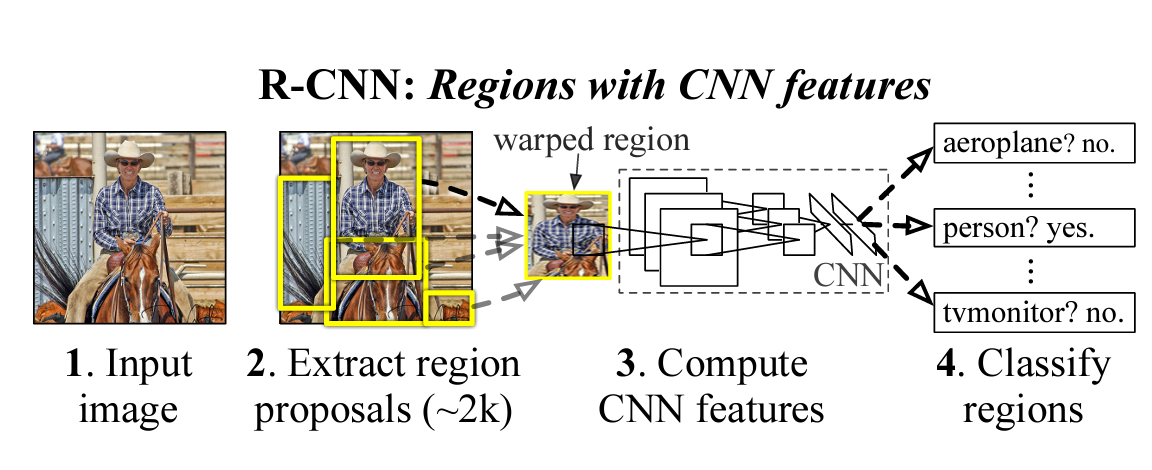
\includegraphics[width=0.6\textwidth]{R_CNN.PNG}
         \caption{R-CNN Model(Source:Girshick et al.)}
            \label{fig:R-CNN Model}
    \end{figure}
\textbf{R-CNN comprises of the following three modules:}\\
        \begin{enumerate}
            \item \textbf{Region proposal: } The R-CNN algorithm starts by identifying regions in an image that may contain objects. These regions are known as region proposals. They are referred to as proposals because they may or may not contain objects, and the goal of the learning function is to remove areas that do not contain objects. These region proposals are essentially bounding boxes around the objects.
            \item \textbf{Feature extraction:} To identify objects in an image, the first step is to crop out the region proposals and resize them. These resized images are then sent through a standard CNN for feature extraction. The original research paper employed AlexNet for this purpose. The CNN extracts 4,096-dimensional feature vectors from each region.
            \item  \textbf{Classifier: } The extracted features are classified by using the standard classification algorithms, such as the linear SVM model 
        \end{enumerate}
R-CNN was the first successful deep learning–based object detection system, but it suffered a serious issue with respect to performance. Its time performance problem is because of the following:
    \begin{itemize}
         \item For feature extraction, each region proposal undergoes approximately 2,000 passes per image in the CNN.
        \item Three models are trained: CNN for feature extraction, classifier for image class prediction, and regression for bounding box refinement. Training is compute-intensive, increasing computation time.
        \item Due to the large number of regions, CNN predictions are slow for each proposal.
    \end{itemize}
        
\subsubsection{Fast R-CNN:} To overcome the limitations of R-CNNs, Ross Girshick from Microsoft published a paper in 2015 titled “Fast R-CNN” that proposed a single model to learn and output regions and classifications directly \href{https://arxiv.org/pdf/1504.08083.pdf}{\textcolor{blue}{Fast R-CNN:}}
\href{https://medium.com/alegion/deep-learning-for-object-detection-and-localization-using-fast-r-cnn-85d52e3928a1}{\textcolor{blue}{[2]}}\\
On the contrary, Fast R-CNN trains a deep VGG-16 network, 9x faster than R-CNN and 213x faster at test time, achieving a higher mAP on PASCAL VOC 2012. How does it achieve this enormous gain in speed? Fast R-CNN evaluates the network and extracts features for the whole image once, instead of extracting features from each RoI, which are cropped and rescaled every time in R-CNN. It then uses the concept of RoI pooling, a special case of pyramid pooling used in SPPNet, to give a feature vector of the desired length. This feature vector is then used for classification and localization. This method is more effective than R-CNN because the computations for overlapping regions are shared.
        

\textbf{Building blocks of Fast R-CNN:}
    \begin{enumerate}
        \item Region proposal network
        \item Feature extraction using CNN
        \item RoI pooling layer: This is where the real magic of Fast R-CNN happens
        \item Classification and Localization
    \end{enumerate}
        
    \begin{figure}[H]
        \centering
        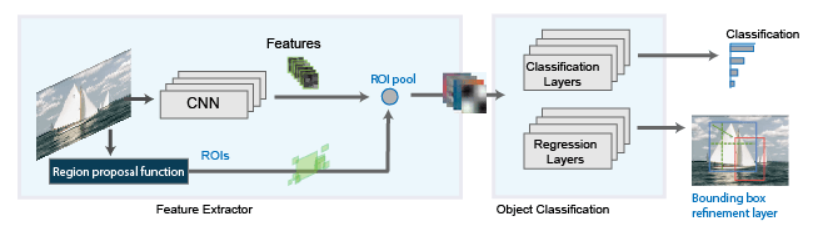
\includegraphics[width=1\textwidth]{Fast_RCNN_ARch.PNG}
        \caption{Architectural Design of Fast R-CNN }
        \label{fig: Fast R-CNN}
    \end{figure}
\href{https://www.mathworks.com/help/vision/ug/getting-started-with-r-cnn-fast-r-cnn-and-faster-r-cnn.html#d117e11449}{\textcolor{blue}{Image Source}}
        
The region proposal network and feature extraction modules are very similar to what we have seen in R-CNN. But instead of passing each cropped and re-scaled RoI, the entire input image is passed through a feature extractor like VGG-16 to produce a convolutional feature map. The features (i.e., the convolutional feature map) are combined with the region proposal network, which uses an SS approach, to form a fixed-length feature vector in the RoI pooling layer. Each of these feature vectors is then passed along to the classification and localization modules. The classification module classifies K+1 (1 for background) object classes using a softmax probability. The localization module outputs four real-valued numbers for each K object class. \cite{girshick2015fast}
\subsubsection{Faster R-CNN}
Faster R-CNN is an improved version of Fast R-CNN from the training speed and detection accuracy perspectives.
Faster R-CNN added what they called a Region Proposal Network (RPN) in an attempt to get rid of the selective search algorithm and make the model completely trainable end-to-end.

\begin{figure}[H]
    \centering
    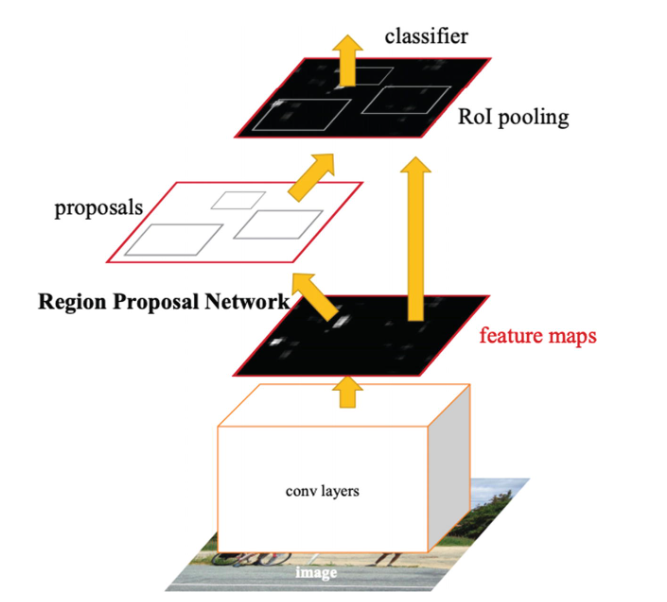
\includegraphics[width=0.7\textwidth]{Faster_RNN.PNG}
    \caption{Architectural Design of Faster R-CNN}
    \label{fig:Faster R-CNN}
\end{figure}

\begin{enumerate}
    \item \textbf{Region Proposal Network: } An RPN is a fully convolutional neural network that predicts object bounds and objectness scores simultaneously at each position of the image.
    An RPN is a deep CNN that takes an image input and generates the output as a set of rectangular object proposals. Each rectangular proposal has an “objectness” score.
    
    \begin{figure}[H]
        \centering
        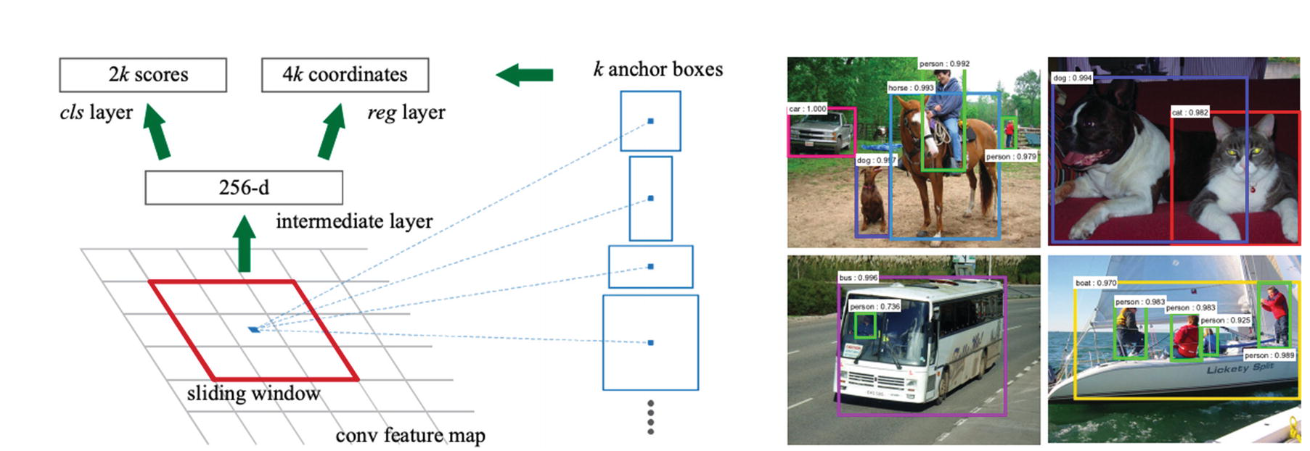
\includegraphics[width=1\textwidth]{RPN.PNG}
        \caption{Region Proposal Networks (RPN) [image source: Shaoqing Ren, et al.]}
        \label{fig:RPN}
    \end{figure}
    RPN has a classifier and a regressor. The authors have introduced the concept of anchors. The anchor is the central point of the sliding window.
    The classifier determines the probability of a proposal having the target object. Regression
    regresses the coordinates of the proposals.
    Multiple region proposals are predicted at each sliding window location. Assuming the maximum number of proposals at each window location is k, the total number of bounding box coordinates will be 4k, and the number of object classes will be 2k (one for the probability of being an object and the other for the probability of not being an object). These region boxes at each window are called anchors.\\
    \item \textbf{Fast R-CNN: } The second part of the faster R-CNN is the detection network. This part is exactly the same as the Fast R-CNN (as described earlier). The Fast R-CNN takes input from the RPN to detect objects in images. 
\end{enumerate} \cite{ansari2020building}, \cite{salvador2016faster}


\subsubsection{Mask R-CNN}
\textcolor{red}{\href{https://arxiv.org/pdf/1703.06870.pdf}{\textcolor{blue}{Mask R-CNN}}}
The Mask R-CNN extends the Faster R-CNN. The Mask R-CNN adds an extra branch for predicting an object mask along with the object class and bounding box coordinates.
Here is how the Mask R-CNN differs from its predecessor, the Faster R-CNN:
\begin{itemize}
    \item The Faster R-CNN has two outputs: a class label and bounding box coordinates.
    \item The Mask R-CNN has three outputs: a class label, bounding box coordinates, and an object mask.
\end{itemize}
In the Mask R-CNN, each pixel is classified into a fixed set of categories without differentiating object instances. It introduces a concept called pixel-to-pixel alignment between the output and input layers of the neural network. The class of each pixel determines the masks in the ROI.

\begin{figure}[H]
    \centering
    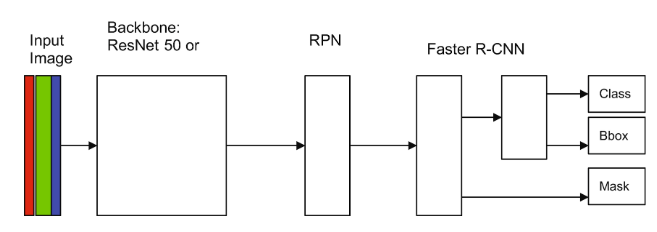
\includegraphics[width=1\textwidth]{MaskR-CNN.PNG}
    \caption{Mask R-CNN network architecture}
    \label{fig:MaskR-CNN}
\end{figure}
As shown in Figure \ref{fig:MaskR-CNN}, the network consists of three components \textbf{modules—backbone, RPN, and output head}.
\begin{itemize}
    \item \textbf{Backbone} The backbone networks are commonly seen in object detection model architectures. The original paper describes using ResNet-50 and ResNet-101[ \textcolor{red}{\href{https://arxiv.org/pdf/1612.03144.pdf}{Ref1}} ]
    The backbone’s main role is feature extraction.
    In addition to ResNet, a feature pyramid network (FPN) is used to extract the finer feature details of the image.
    \begin{figure}[H]
        \centering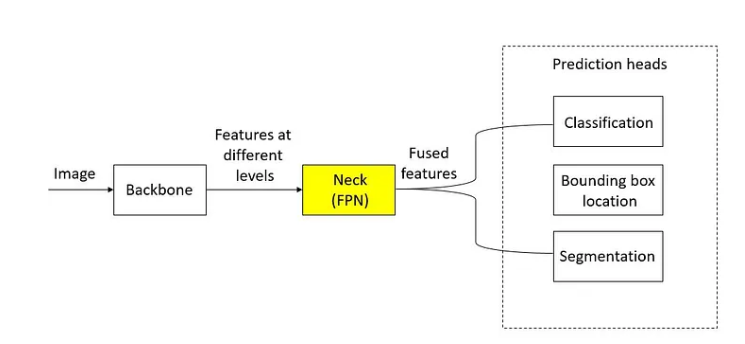
\includegraphics[width=1\textwidth]{BackBone_FPN.PNG}
        \caption{BackBone and FPN Tuning architecture \protect\href{https://medium.com/@freshtechyy/fusing-backbone-features-using-feature-pyramid-network-fpn-c652aa6a264b}{[\textcolor{blue}{Ref}} ]}
    \end{figure}
The FPN consists of decreasing-size layers of a CNN, in which case each forward layer has fewer neurons.

        \item \textbf{Feature Pyramid Network (FPN): } is a neck network that combines features of different resolutions obtained from a backbone network, such as ResNet. A CNN-based backbone applies convolution layers to an input image, which results in a set of feature maps with decreasing resolution due to pooling or convolution with a stride different from one.\\
        The FPN includes a bottom-up pathway and a top-down pathway. In the bottom-up pathway, a backbone network, like ResNet, is used to perform feature extraction to extract features with decreasing levels of spatial resolution.
        As the levels of resolution decrease, the semantic meaning of the feature maps increases, as indicated by the thickness of box boundaries in blue.\\
        In the top-down pathway, the feature maps are fused to have both rich semantic meaning and accurate spatial information as shown in the figure \ref{fig:FPN_Arch} below.
        \begin{figure}[H]
            \centering
            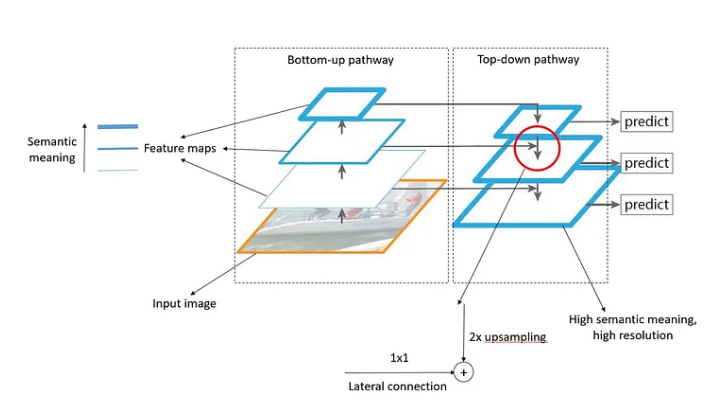
\includegraphics[width=0.7\textwidth]{FPN_Top_bott.PNG}
            \caption{Feature Pyramid Network (FPN)}
            \label{fig:FPN_Arch}
        \end{figure}
         \item \textbf{Output Head: } The last module consists of the Faster R-CNN with an additional output branch. \cite{he2017mask}
\end{itemize}
   
\subsection{One stage detector: } 
They can process images in real-time and are suitable for applications where low latency is crucial, such as real-time object detection in video streams or robotics.

\subsubsection{Single-Shot Multibox Detection: }

SSD is designed for object detection in real time. An R-CNN and its variants are detectors that work in two stages. They have two specialized networks: one network creates the region proposals to predict bounding boxes, and the other network predicts the object classes. These detectors are fairly accurate, but they come with a high computational cost. As a result, they are not suitable for detecting objects in real-time streaming videos.
A single-shot object detector predicts both the bounding boxes and the object classes in a single forward pass of the network.\cite{liu2016ssd} \href{https://arxiv.org/pdf/1512.02325.pdf}{\textcolor{blue}{[Original Paper]}}
\begin{itemize}
    \item \textbf{SSD Network Architecture: } The SSD approach is a method that uses a feed-forward convolutional network to generate a set of fixed-size bounding boxes and scores, which helps detect the presence of object class instances in those boxes. In the final stage, a non-maximum suppression step is performed to obtain the ultimate detections. \\
    \begin{itemize}
        \item \textbf{Grid cell: } Instead of using sliding window, SSD divides the image using a grid and has each grid cell be responsible for detecting objects in that region of the image. Detection of objects simply means predicting the class and location of an object within that region. If no object is present, we consider it the background class, and the location is ignored. 
        SSD only needs an input image and ground truth boxes for each object during training.
        In a convolutional fashion, we evaluate a small set
        of default boxes of different aspect ratios at each location in several feature maps with
        different scales (e.g. 8x8 and 4x4 in (b) and (c)). For each default box, we predict
        both the shape offsets and the confidences for all object categories ((c1; c2; ...; cp)).
        At training time, we first match these default boxes to the ground truth boxes.
        \begin{figure}[H]
            \centering
            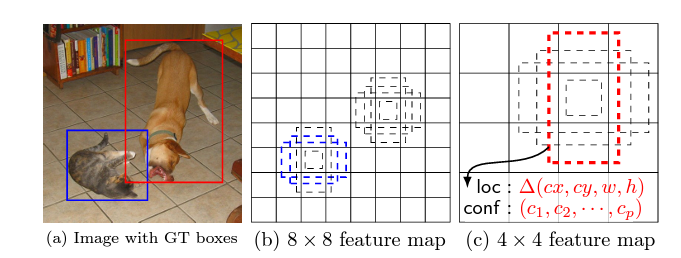
\includegraphics[width=\textwidth]{SSD_GridCell.PNG}
            \caption{SSD:Single Shot Multi Box Detector \textcolor{red}{\protect\href{https://arxiv.org/pdf/1512.02325.pdf}{image source}}}
            \label{fig:SSD_grid}
        \end{figure}
        
        \item \textbf{Anchor Boxes:} In object detection, we are seeking to identify and localize objects as they appear in an image. Object detection differs from image classification because there may be multiple objects of the same or different classes present in the image, and object detection seeks to accurately predict all of these objects.
        Object detection models tackle this task by breaking the prediction step into two pieces: 
        \textcolor{red}{\href{https://blog.roboflow.com/what-is-an-anchor-box/}{Ref: Anchor-box}}
        \begin{enumerate}
            \item First, they predict a bounding box through regression and
            \item Second, by predicting a class label through classification.
        \end{enumerate}
        
        \begin{figure}[H]
            \centering
            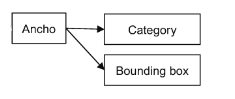
\includegraphics[width=0.2\textwidth]{Anchor.PNG}
            \caption{Anchor}
            \label{fig:anchor}
        \end{figure}
        To predict and localize many different objects in an image, most state-of-the-art object detection models such as SSD, EfficientDet, and the YOLO models start with anchor boxes as a prior, and adjust from there. These anchor boxes are pre-defined, and each one is responsible for a size and shape within a grid cell.
        
        Anchors are one or more rectangular shapes set at each convolution point of the feature map. 
        Each grid cell in SSD can be assigned multiple anchor/prior boxes.
        
        
        In Figure \ref{fig: anchor box}, there are five rectangular anchors (shown in red outlines) set at a point (shown in blue).
        \begin{figure}[H]
            \centering
            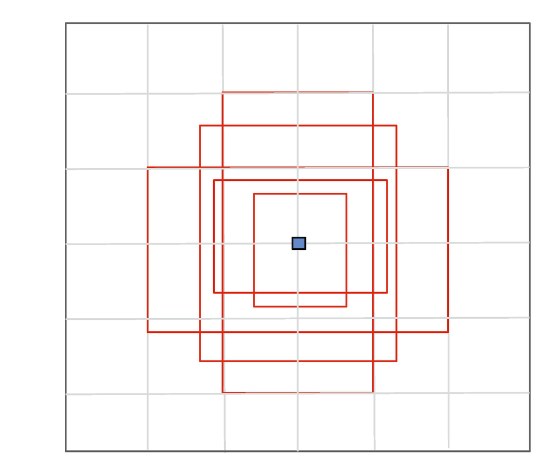
\includegraphics[width=0.5\textwidth]{Anchor_Boxes.PNG}
            \caption{Anchor Boxes}
            \label{fig: anchor box}
        \end{figure}
        In SSD, typically five anchor boxes are selected at each point. Each of these anchors acts as a detector.
        The varying size of these detectors allows them to detect objects of different sizes. Smaller detectors will detect smaller objects, and larger detectors are capable of detecting larger objects.\\
        \item \textbf{Default Boxes and Aspect Ratios: }  doesn’t use k-means to find the anchors. Instead it uses a mathematical formula to compute the anchor sizes. Therefore, SSD’s anchors are independent of the dataset (by the way, the SSD paper calls them “default boxes”)\textcolor{red}{\href{https://arxiv.org/pdf/1512.02325.pdf}{Ref:Original Paper}}.  \href{https://machinethink.net/blog/object-detection/}{SSD}

        It is important to note that these anchors are chosen beforehand as constants. In SSD, a set of fixed “default anchors” is mapped at each convolution point.\\
        They have associated a set of default bounding boxes with each feature map cell, for multiple feature maps at the top of the network. The default boxes tile the feature map in a convolutional manner so that the position of each box relative to its corresponding cell is fixed.\\
            \end{itemize}
    \item \textbf{Model Architecture: } An SSD neural network consists of two components: \textbf{base network and prediction network.}
    \begin{enumerate}
        \item \textbf{Base network:} The base network is a deep convolutional network that is truncated before any classification layer. For example, remove the fully connected layer of ResNet or VGG to create the base network for SSD. The base network is used for feature extraction from the input images.
        \item \textbf{Detection network:} To the base network, attach some extra convolutional layers that will actually do the prediction of bounding boxes and object classes. 
        \begin{figure}[H]
        \centering
        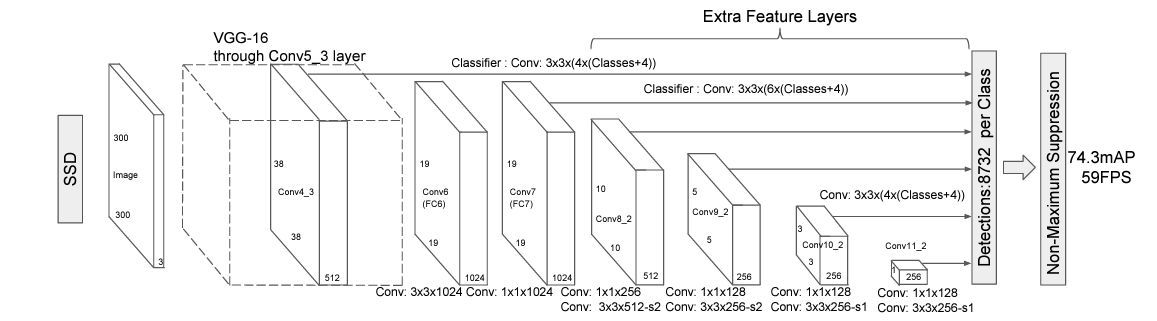
\includegraphics[width=\textwidth]{SSD_ARch.PNG}
        \caption{single shot detection models: SSD \cite{liu2016ssd}}
        \label{fig: single shot detection models: SSD}
        \end{figure}
    The detection network has the following characteristics.
        \begin{itemize}
            \item These layers decrease in size progressively and allow
            predictions of detections at multiple scales
            \item  The convolutional model for predicting detections is different for each feature layer
            \item Each added feature layer (or optionally an existing
            feature layer from the base network) can produce a fixed set of detection predictions
            using a set of convolutional filters.
        \end{itemize}
    \end{enumerate}
    \item \textbf{Matching System: } During training, we need to select default boxes that correspond to ground truth detection and train the network accordingly. For each ground truth box, we choose from default boxes that vary in location, aspect ratio, and scale.  The SSD uses IoU (intersection over union) to match the default boxes with the ground truth. This is done by determining the overlap between them. The IoU-based overlap is also known as the Jaccard overlap. If the overlap between the default box and the ground truth is 0.5 or more, it is considered a match. This process of matching is repeated at each layer, which allows the network to learn at scale. Initially, the SSD uses the default boxes as predictions and then tries to regress and come closer to the ground truth bounding boxes. \cite{ansari2020building}, \cite{liu2016ssd}

\end{itemize}

\subsection{Object Detection Evaluation Metrics}
Object detection is a computer vision task where the goal is to identify and locate objects of interest within an image or a video. Several evaluation metrics are commonly used to assess the performance of object detection algorithms. Here are some of the key metrics:
\subsubsection{Intersection over Union (IoU)}
Intersection over union (IoU), also known as the Jaccard index, is one of the most commonly used evaluation metrics in object detection algorithms. It is used to evaluate the performance of object detection by comparing the ground truth bounding box to the predicted bounding box and IoU.
In object detection, we create training sets by drawing bounding boxes around objects for labeling. These bounding boxes in the training set are also known as the ground truth. During the model learning, the object detection algorithm predicts bounding boxes and compares them against the ground truth. IoU is used to evaluate how closely the predicted bounding box overlaps with the ground truth. \cite{ansari2020building}, \cite{bfortuner_mlglossary}, \cite{liu2016ssd}

\begin{figure}[H]
    \centering
    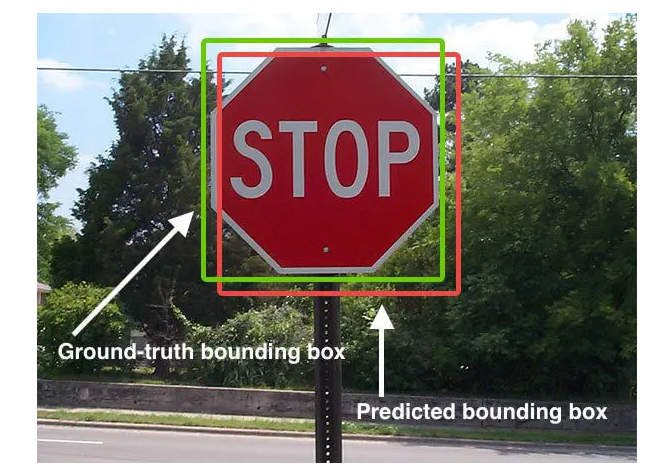
\includegraphics[width=0.6\textwidth]{Intersection_overUnion_(IoU).PNG}
    \caption{The predicted bounding box and Ground-truth bounding box}
    \label{fig:PBGTB}
\end{figure}

\textbf{Computing Intersection over Union can therefore be determined as:}\\

\begin{figure}[H]
    \centering
    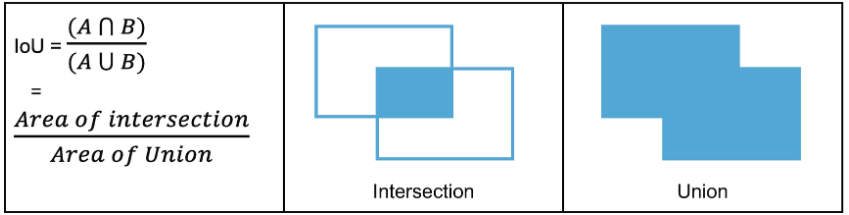
\includegraphics[width=0.6\textwidth]{Intersection_OverUnion.PNG}
    \caption{Intersection OverUnion}
    \label{fig:Intersection_OverUnion}
\end{figure}

\subsubsection{Mean Average Precision (mAP)}

Mean Average Precision (mAP) is commonly used to analyze the performance of object detection and segmentation systems. Many object detection algorithms, such as Faster R-CNN, MobileNet SSD, and YOLO, use mAP to evaluate their models. The mAP is also used across several benchmark challenges, such as Pascal, VOC, COCO, and more. The mean of average precision(AP) values are calculated over recall values from 0 to 1. \cite{padilla2020survey}, \cite{ansari2020building},  \\
mAP formula is based on the following sub metrics:
\begin{itemize}
    \item Confusion Matrix
    \item Intersection over Union(IoU)
    \item Recall,
    \item Precision
\end{itemize}
\begin{enumerate}
    \item \textbf{Confusion Matrix: }A confusion matrix is a table that is often used to evaluate the performance of a classification algorithm on a set of labeled data for which the true values are known. It provides a summary of the classification results, breaking down the predicted and actual classes into four categories: true positives (TP), true negatives (TN), false positives (FP), and false negatives (FN). \cite{padilla2020survey}, \cite{li2019analysis}
    \begin{itemize}
        \item \textbf{True Positives (TP): } The model predicted a label and matches correctly as per ground truth.\\
        \item \textbf{True Negatives (TN): } The model does not predict the label and is not a part of the ground truth.\\
        \item  \textbf{False Positives (FP): } The model predicted a label, but it is not a part of the ground truth (Type I Error).\\
        \item \textbf{False Negatives (FN): } The model does not predict a label, but it is part of the ground truth. (Type II Error).
        \begin{figure}[H]
            \centering
            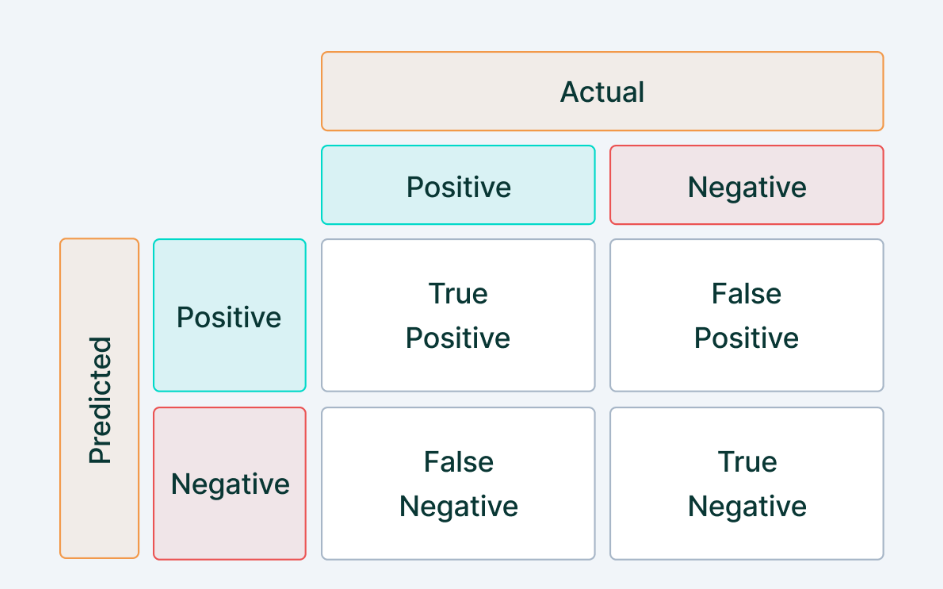
\includegraphics[width=0.7\textwidth]{confusion_matrix.PNG}
            \caption{Confusion matrix table}
            \label{fig:Confusion_Matrix}
        \end{figure}
    \end{itemize}
    \item \textbf{Precision: } Precision measures how well you can find true positives(TP) out of all positive predictions. (TP+FP).
    $$Precision=\frac{TP}{TPTP+FP}$$

    \item \textbf{Recall: } Recall measures how well you can find true positives(TP) out of all predictions(TP+FN).
    $$Recall=\frac{TP}{TPTP+FN}$$
    
  
\end{enumerate}


\subsection{YOLO}
YOLO is a real-time object detection algorithm that is designed to be fast and accurate. It uses a single convolutional neural network to simultaneously predict the bounding boxes and class probabilities of objects in an image. What sets YOLO apart from other object detection algorithms is that it trains on the full image and is set up to solve regression problems. This means that it does not require a complex processing pipeline, which makes it extremely fast.YOLO is a system that simplifies object detection by treating it as a single regression problem. It predicts bounding box coordinates and class probabilities directly from image pixels. With YOLO, you can detect objects in an image with just one look and get information about what objects are present and where they are located. \cite{redmon2016you}, \cite{ansari2020building}

\subsubsection{Detection Algorithm}
The YOLO design enables end-to-end training and real-time speeds while maintaining high average precision. \\
It divides the image into an SxS grid and for each
grid cell predicts \textbf{B} bounding boxes, confidence for those boxes,
and C-class probabilities. These predictions are encoded as a tensor.
\[
S x S x (B*5 + C)
\]
\\
\begin{figure}[H]
    \centering
    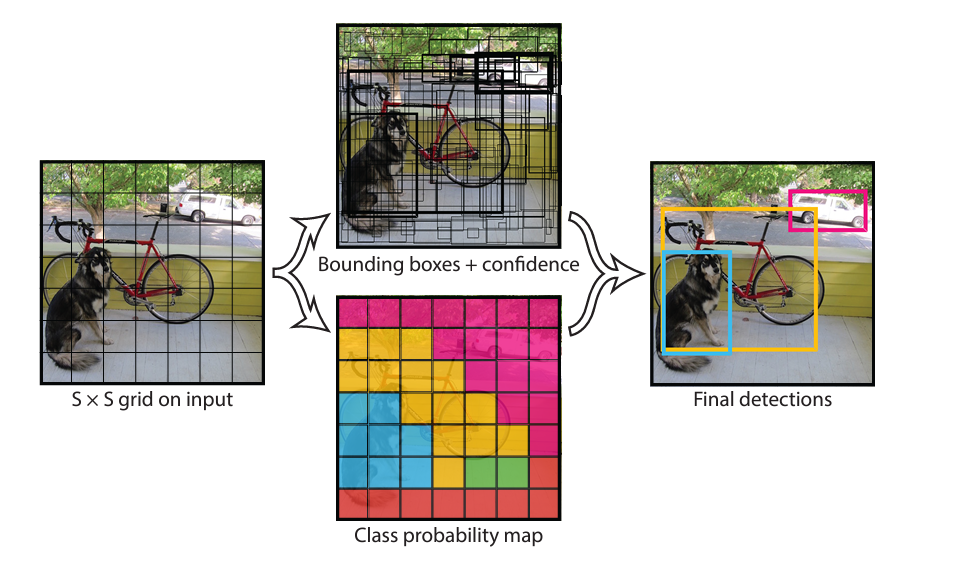
\includegraphics[width=0.8\textwidth]{YOLO_Detection.PNG}
    \caption{YOLO Model}
    \label{fig:YoloV1_Model}
\end{figure}

Each bounding box consists of 5 predictions: x, y, w, h,
and confidence. confidence scores reflect how confident the model is.
\[
Confidence =Pr(Object)*IOU_{pred}^{truth}
\]
\subsubsection{YOLO Architectural Design}
The YOLO network architecture takes inspiration from the GoogLeNet model that is used for image classification. It consists of 24 convolutional layers followed by 2 fully connected layers. In contrast to the inception modules used in GoogLeNet, the YOLO network employs 1x1 reduction layers that are then followed by 3x3 convolutional layers. The full network is shown in Figure[\ref{fig:YOLO_arc}].
\begin{figure}[H]
    \centering
    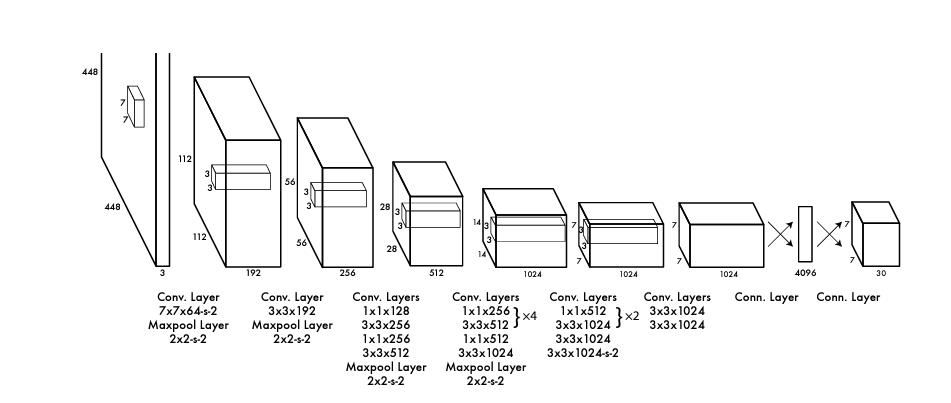
\includegraphics[width=\textwidth]{Yolo_Arch.PNG}
    \caption{YOLO Model}
    \label{fig:YOLO_arc}
\end{figure}
The convolutional layers were pre-trained on the ImageNet 1000-class competition dataset. For pretraining, YOLO uses the first 20 convolutional layers from Figure \ref{fig:YOLO_arc}, followed by an average-pooling layer and a fully connected layer. The final layer predicts both class probabilities and bounding box coordinates. A linear activation function is used for the final layer and
all other layers use the following leaky rectified linear activation:
 \[
 \phi(x)=\begin{cases}
           x, & \text{if } x>0 \\
          0.1x, & \text{otherwise}
      \end{cases}
\]

\subsubsection{Limitations of YOLO}
\begin{itemize}
    \item It struggles with small objects that come in groups, such as flocks of birds.
    \item It can predict only one class of objects within a cell grid.
    \item It does not predict well if the object has an unusual aspect ratio that was not seen in the training set.
    \item Its accuracy is less than some of the state-of-the-art algorithms, such as the Faster R-CNN
\end{itemize}

\subsection{Transfer Learning and Pre-trained Models:}

Transfer learning is a technique in deep learning where a pre-trained model for a particular task is used as a starting point for another model that performs a similar task. This approach provides a faster and easier way to update and retrain a network as compared to training a network from scratch. It is commonly used in various applications, such as object detection, image recognition, and speech recognition. \cite{you2021logme}
\href{https://www.mathworks.com/discovery/transfer-learning.html?s_tid=srchtitle_support_results_1_Transfer%2520Learning}{\textcolor{blue}{Source Matlab}}

Transfer learning is a popular technique because:
\begin{itemize}
    \item It enables you to train models with less labeled data by reusing popular models that have already been trained on large datasets.
    \item  It can reduce training time and computing resources. With transfer learning, the weights are not learned from scratch because the pre-trained model has already learned the weights based on previous learning.
    \item You can take advantage of model architectures developed by the deep learning research community, including popular architectures such as GoogLeNet and ResNet.
\end{itemize}
\begin{figure}[H]
    \centering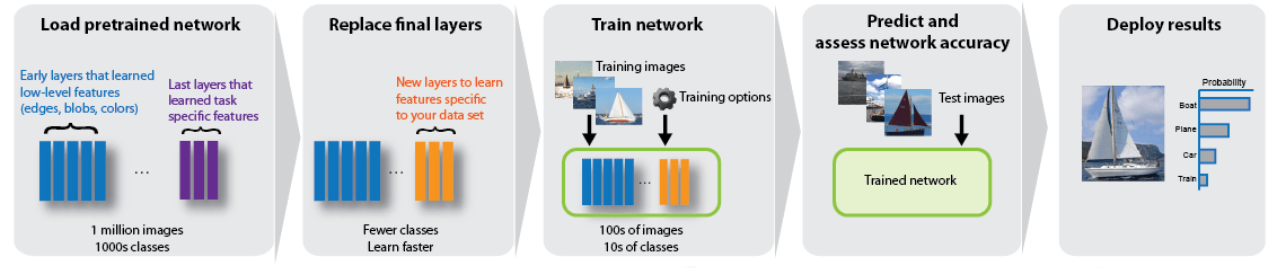
\includegraphics[width=1\linewidth]{Transfer_Learning_Model.PNG}
    \caption{Transfer Learning \protect\href{https://www.mathworks.com/help/deeplearning/ug/pretrained-convolutional-neural-networks.html}{\textcolor{blue}{Image source}}}
    \label{fig:Transfer Learning}
\end{figure}
\subsubsection{Pre-trained Model}
There are several pre-trained models available for object detection. Below are some of the most popular ones:\\
\begin{itemize}
    \item Alexnet, googlenet(ImageNet), goolgenet(Places365), resnet18, resnet50, resnet101, vgg16, vgg19, inceptionv3, inceptionresnetv2, squeezenet, densenet201, mobilenetv2, shufflenet, xception, nasnetmobile, nasnetlarge. 
\end{itemize}

When choosing a neural network, it is important to consider its accuracy, speed, and size, as these are the most crucial characteristics. Typically, there is a tradeoff between these factors. To make an informed decision, you can refer to the plot below, which compares the ImageNet validation accuracy with the time taken to make a prediction using the neural network. \cite{li2019analysis}
\begin{figure}[H]
    \centering
    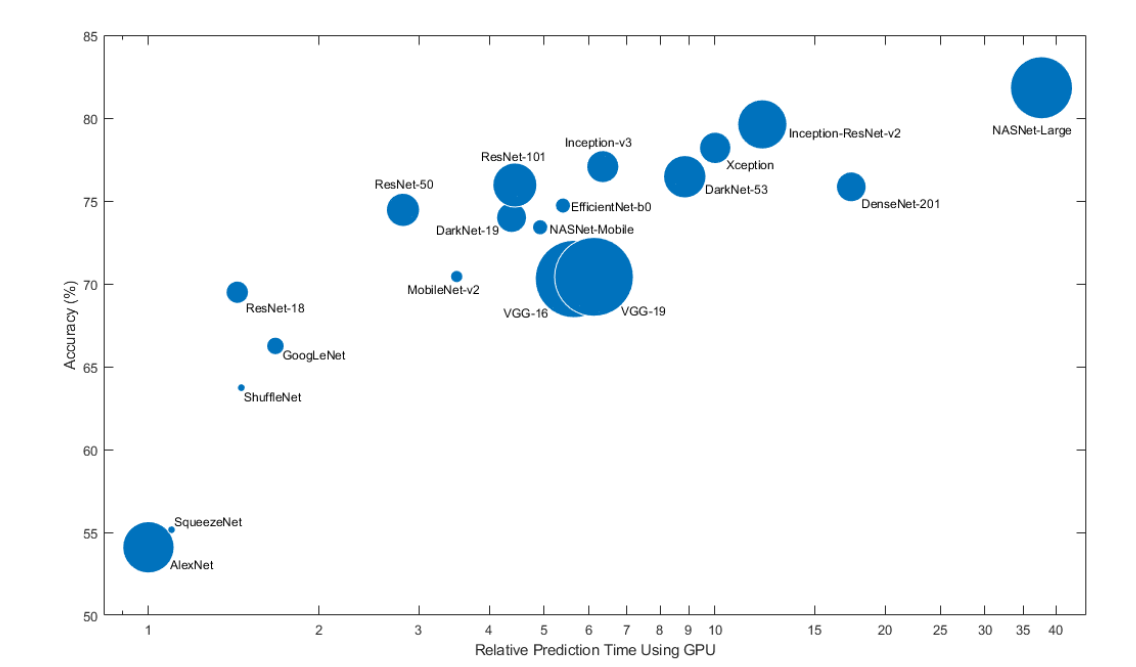
\includegraphics[width=1\textwidth]{Pre-trained_comparision.PNG}
    \caption{Compare Pretrained Neural Networks}
    \label{fig: Pretrained Model Comparison}
\end{figure}

